\documentclass{beamer}

\usepackage{amsmath}
\usepackage{graphicx}
\usepackage{subcaption}

\usetheme{AnnArbor}
\usecolortheme{crane}
\usefonttheme[onlymath]{serif}

\title{Deep Learning - Foundations and Concepts}
\subtitle{Chapter 6. Deep Neural Networks}
\author{nonlineark@github}
\date{\today}

\begin{document}

\begin{frame}
    \titlepage
\end{frame}

\begin{frame}
    \frametitle{Outline}
    \tableofcontents
\end{frame}

\section{Limitations of Fixed Basis Functions}

\begin{frame}
    \frametitle{The curse of dimensionality}
    In spaces of higher dimensionality, the number of combinations of values must be considered could be huge. This effect is known as combinatorial explosion:
    \begin{itemize}
        \item A polynomial regression of order $M$ for a single input variable needs $M+1$ parameters. If there are $D$ input variables, the number of parameters needed will be $\binom{M+D}{M}$.
        \item The histogram based classification for $1$-dimensional input needs $N$ buckets. If the input is $D$-dimensional, the number of buckets needed will be $N^{D}$.
    \end{itemize}
    For a machine learning model, this usually means that the amount of data needed to generlize accurately grows exponentially.
\end{frame}

\begin{frame}
    \frametitle{High-dimensional spaces}
    High-dimensional spaces can defeat one's geometrical intuitions:
    \begin{itemize}
        \item In spaces of high dimensionality, most of the volume of a hypersphere is concentrated in a thin shell near the surface.
        \item In spaces of high dimensionality, the probability mass of the Gaussian is concentrated in a thin shell at a specific radius (a soap bubble).
    \end{itemize}
\end{frame}

\begin{frame}
    \frametitle{Data manifolds}
    Although data may be in high-dimensional spaces, real data will generally be confined to a region of the data space having lower effective dimensionality. Effectively, neural networks learn a set of basis functions that are adpated to data manifolds.
\end{frame}

\begin{frame}
    \frametitle{Data manifolds}
    \begin{figure}
        \caption{Images of a handwritten digit that lives on a nonlinear three-dimensional manifold}
        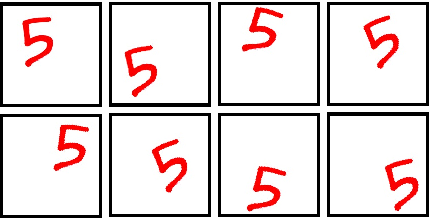
\includegraphics{Figure_7.pdf}
    \end{figure}
\end{frame}

\begin{frame}
    \frametitle{Data manifolds}
    \begin{figure}
        \caption{Natural images vs. randomly generated images}
        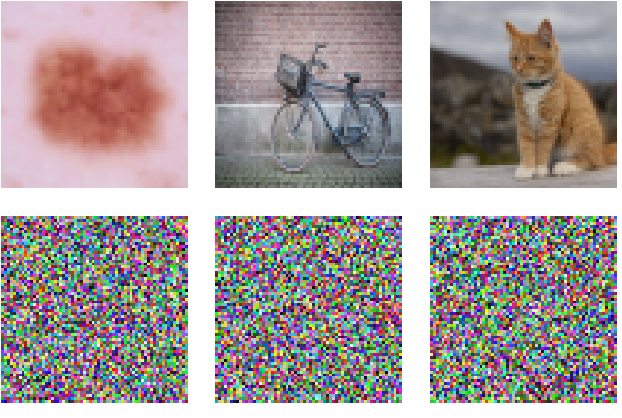
\includegraphics[height=0.7\textheight]{Figure_8.pdf}
    \end{figure}
\end{frame}

\begin{frame}
    \frametitle{Data-dependent basis functions}
    \begin{itemize}
        \item Simple basis functions that are chosen independently of the problem being solved can run into significant limitations.
        \item Using expert knowledge to hand-craft the basis functions was superseded by data-driven approaches in which basis functions are learned from the training data.
        \item Methods such as radial basis functions and support vector machines have been superseded by deep neural networks, which are much better at exploiting very large data sets efficiently.
    \end{itemize}
\end{frame}

\section{Multipayer Networks}

\begin{frame}
    \frametitle{Parameter matrices}
    Consider a basic neural network model having two layers of learnable parameters:
    \begin{align*}
        a_{m}^{(1)}&=\sum_{d=1}^{D}w_{md}^{(1)}x_{d}+w_{m0}^{(1)} \\
        z_{m}^{(1)}&=h(a_{m}^{(1)}) \\
        a_{k}^{(2)}&=\sum_{m=1}^{M}w_{km}^{(2)}z_{m}^{(1)}+w_{k0}^{(2)}
    \end{align*}
    where $h$ is a differentiable, nonlinear activation function.
\end{frame}

\begin{frame}
    \frametitle{Parameter matrices}
    \begin{figure}
        \caption{Network diagram for a two-layer neural network}
        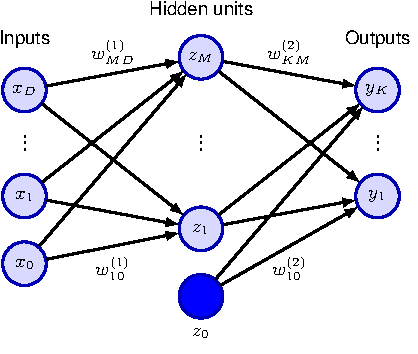
\includegraphics{Figure_9.pdf}
    \end{figure}
\end{frame}

\begin{frame}
    \frametitle{Parameter matrices}
    The bias parameters can be absorbed into the set of weight parameters, so the two-layer neural network can be represented as:
    \begin{align*}
        y_{k}(x;w)&=f(\sum_{m=0}^{M}w_{km}^{(2)}h(\sum_{d=0}^{D}w_{md}^{(1)}x_{d})) \\
        y(x;w)&=f(W^{(2)}h(W^{(1)}x))
    \end{align*}
    where $f$ and $h$ are activation functions evaluated on each vector element separately.
\end{frame}

\begin{frame}
    \frametitle{Universal approximation}
    \begin{itemize}
        \item For a wide range of activation functions, two-layer feed-forward networks can approximate any function defined over a continuous subset of $\mathbb{R}^{D}$ to arbitrary accuracy.
        \item However, in a practical application, there can be huge benefits in considering networks having many more than two layers that can learn hierarchical internal representations.
    \end{itemize}
\end{frame}

\begin{frame}
    \frametitle{Universal approximation}
    \begin{figure}
        \caption{Two-layer neural networks are universal approximators}
        \begin{subfigure}{0.7\textwidth}
            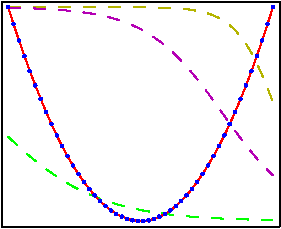
\includegraphics[width=0.45\textwidth]{Figure_10_a.pdf}
            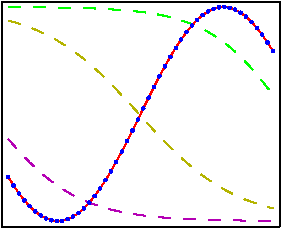
\includegraphics[width=0.45\textwidth]{Figure_10_b.pdf}
        \end{subfigure}
        \begin{subfigure}{0.7\textwidth}
            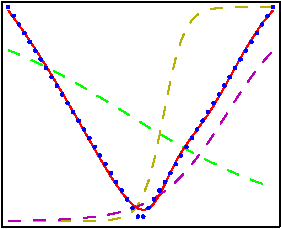
\includegraphics[width=0.45\textwidth]{Figure_10_c.pdf}
            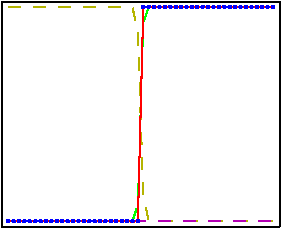
\includegraphics[width=0.45\textwidth]{Figure_10_d.pdf}
        \end{subfigure}
    \end{figure}
\end{frame}

\begin{frame}
    \frametitle{Hidden unit activation functions}
    \begin{itemize}
        \item Activation functions for the output units are determined by the kind of distribution being modelled.
        \item For the hidden units, the only requirement is that they need to be differentiable.
        \item Obviously, the identity function, sometimes used as the activation function for output units, is not a good option for hidden units.
    \end{itemize}
\end{frame}

\begin{frame}
    \frametitle{Hidden unit activation functions}
    \begin{figure}
        \caption{A variety of nonlinear activation functions}
        \begin{subfigure}{0.8\textwidth}
            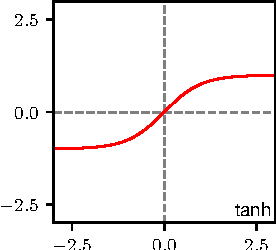
\includegraphics[width=0.3\textwidth]{Figure_12_a.pdf}
            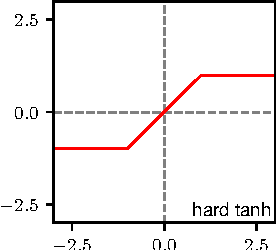
\includegraphics[width=0.3\textwidth]{Figure_12_b.pdf}
            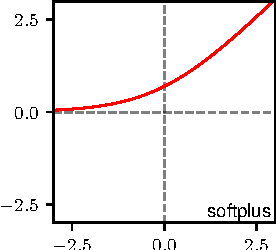
\includegraphics[width=0.3\textwidth]{Figure_12_c.pdf}
        \end{subfigure}
        \begin{subfigure}{0.8\textwidth}
            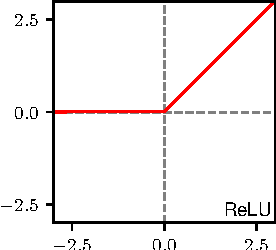
\includegraphics[width=0.3\textwidth]{Figure_12_d.pdf}
            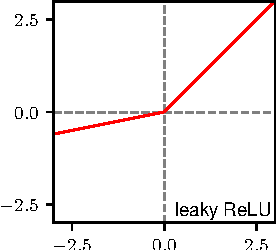
\includegraphics[width=0.3\textwidth]{Figure_12_e.pdf}
            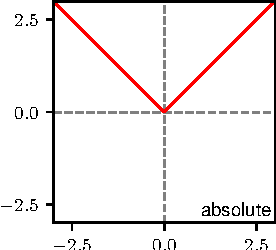
\includegraphics[width=0.3\textwidth]{Figure_12_f.pdf}
        \end{subfigure}
    \end{figure}
\end{frame}

\begin{frame}
    \frametitle{Weight-space symmetries}
    Consider a two-layer network with $M$ hidden units having $\tanh$ activation functions and full connectivity in both layers:
    \begin{itemize}
        \item Changing the sign of all the weights and the bias feeding into a particular hidden unit can be compensated by changing the sign of all the weights leading out of that hidden unit:
        \begin{itemize}
            \item $2^{M}$ equivalent weight vectors.
        \end{itemize}
        \item Interchange a particular hidden unit with a different hidden unit:
        \begin{itemize}
            \item $M!$ equivalent weight vectors.
        \end{itemize}
    \end{itemize}
\end{frame}

\end{document}